% Template for ICASSP-2017 paper; to be used with:
%          spconf.sty  - ICASSP/ICIP LaTeX style file, and
%          IEEEbib.bst - IEEE bibliography style file.
% --------------------------------------------------------------------------
\documentclass{article}
\usepackage{spconf,amsmath,graphicx}
\usepackage{subcaption}
\usepackage{tikz}
\usepackage{tabularx}
\usepackage{booktabs}
\usetikzlibrary{calc,chains,shapes,positioning,patterns}
\usepackage{phaistos}
\usepackage{pgfplots}
\usepackage{cite}
% Example definitions.
% --------------------
\def\x{{\mathbf x}}
\def\L{{\cal L}}

% Title.
% ------
\title{LATE REVERBERANT POWER SPECTRAL DENSITY ESTIMATION \\ BASED ON AN EIGENVALUE DECOMPOSITION}
%
% Single address.
% ---------------
\name{Ina Kodrasi, Simon Doclo
\thanks{
This work was supported in part by the Cluster of Excellence 1077 ``Hearing4All'', funded by the German Research Foundation (DFG), the Marie Curie Initial Training Network DREAMS (Grant no. 316969), and the joint Lower Saxony-Israeli Project ATHENA, funded by the State of Lower Saxony.
}}
\address{
University of Oldenburg, Department of Medical Physics and Acoustics,  \\ and Cluster of Excellence Hearing4All, Oldenburg, Germany \\
{\tt \{ina.kodrasi,simon.doclo\}@uni-oldenburg.de}\\
}
\begin{document}
\newlength\figureheight
\newlength\figurewidth
\setlength\figureheight{1.9cm}
\setlength\figurewidth{0.4\textwidth}
\ninept
%
\maketitle
%
\begin{abstract}
  Multi-channel methods for estimating the late reverberant power spectral density~(PSD) rely on an estimate of the direction of arrival~(DOA) of the speech source or of the relative early transfer functions~(RETFs) of the target signal from a reference microphone to all microphones.
  The DOA and the RETFs may be difficult to estimate accurately, particularly in highly reverberant and noisy scenarios.
  In this paper we propose a novel multi-channel method to estimate the late reverberant PSD which does not require estimates of the DOA or RETFs. 
The late reverberation is modeled as an isotropic sound field and the late reverberant PSD is estimated based on the eigenvalues of the prewhitened received signal PSD matrix.
Experimental results demonstrate the advantages of using the proposed estimator in a multi-channel Wiener filter for speech dereverberation, outperforming a recently proposed maximum likelihood estimator both when the DOA is perfectly estimated as well as in the presence of DOA estimation errors. 
\end{abstract}
%
\begin{keywords}
speech dereverberation, MWF, late reverberant PSD, EVD, prewhitening
\end{keywords}
%
\section{Introduction}
\label{sec:intro}

In many speech communication applications the received microphone signals are corrupted by reverberation, typically leading to decreased speech quality and intelligibility~\cite{Beutelmann_2006,Goetze_AES_2010,Warzybok_IWAENC_2014} and performance deterioration in speech recognition systems~\cite{Yoshioka_ISPM_2012,Xiong_EURASIP_2015}. 
Since late reverberation is the major cause of speech quality and intelligibility degradation, effective enhancement techniques that reduce the late reverberation are required.
In the last decades many single- and multi-channel dereverberation techniques have been proposed~\cite{Naylor_Derev_book}, with multi-channel techniques being generally preferred since they exploit both the spectro-temporal and the spatial characteristics of the received microphone signals.
Many such techniques require an estimate of the late reverberant power spectral density~(PSD), e.g.,~\cite{Braun_EUSIPCO_2013,Kuklasinski_EUSIPCO_2014g,OSchwartz_ITASLP_2015}.
The late reverberant PSD can be estimated using single- or multi-channel estimators, with multi-channel estimators shown to yield a higher PSD estimation accuracy~\cite{Jensen_ICASSP_2015}.

Dual-channel coherence-based estimators are proposed in e.g.,~\cite{Thiergart_JASA_2012,ASchwarz_ITASLP_2015}, which however exploit only two microphones.
A multi-channel maximum likelihood~(ML) estimator is proposed in~\cite{Braun_EUSIPCO_2013}, where the late reverberation is modeled as an isotropic sound field and the late reverberant PSD is estimated from a set of reference signals at the output of a blocking matrix.
In~\cite{Kuklasinski_EUSIPCO_2014g} the use of a blocking matrix is circumvented and an ML estimate of the late reverberant PSD is derived from the received microphone signals.
In~\cite{Kuklasinksi_ICASSP_2015}, it is theoretically and experimentally validated that the ML estimator proposed in~\cite{Kuklasinski_EUSIPCO_2014g} yields a higher PSD estimation accuracy than the ML estimator proposed in~\cite{Braun_EUSIPCO_2013}.
While a noise-free scenario is assumed in~\cite{Kuklasinski_EUSIPCO_2014g}, late reverberant PSD estimators for noisy scenarios are proposed in~\cite{Braun_EUSIPCO_2013,Braun_EURASIP_2015,Schwartz_WASPAA_2015,Schwartz_ICASSP_2016,Kuklasinski_ITASLP_2016}.
All multi-channel late reverberant PSD estimators in~\cite{Braun_EUSIPCO_2013,Kuklasinski_EUSIPCO_2014g,Braun_EURASIP_2015,Schwartz_WASPAA_2015,Schwartz_ICASSP_2016,Kuklasinski_ITASLP_2016} require an estimate of the direction of arrival~(DOA) of the speech source or of the relative early transfer functions~(RETFs) of the target signal from a reference microphone to all microphones.
The DOA and the RETFs may be difficult to estimate accurately, particularly in highly reverberant and noisy scenarios.
As is experimentally validated in~\cite{ASchwarz_ITASLP_2015, kuklasinski_AES_2016}, DOA estimation errors degrade the PSD estimation accuracy, yielding as a result a degradation in the dereverberation performance of the used speech enhancement system.

In this paper a novel multi-channel late reverberant PSD estimator is proposed, which does not require knowledge of the DOA or RETFs. 
The late reverberation is modeled as an isotropic sound field and the late reverberant PSD is estimated based on the eigenvalues of the prewhitened received signal PSD matrix.
Experimental results demonstrate the advantages of using the proposed estimator in a multi-channel Wiener filter~(MWF) for speech dereverberation, outperforming the ML estimator in~\cite{Kuklasinski_EUSIPCO_2014g} both when the DOA is perfectly estimated as well as in the presence of DOA estimation errors. 

% A commonly used speech enhancement technique is multi-channel Wiener filtering~(MWF), which yields a minimum mean square error estimate of the target dereverberated signal~\cite{}.
% In order to implement the MWF in this setup, the spatial coherence matrix of the late reverberation as well as an estimate of the late reverberant power spectral density~(PSD) is required.
% The spatial coherence matrix is typically computed by modelling the late reverberation as a spherically or cylindrically isotropic sound field~\cite{Braun_EUSIPCO_2013,Kuklasinski_EUSIPCO_2014g,Braun_EURASIP_2015,OSchwartz_ITASLP_2015,kuklasinski_AES_2016,Schwartz_ICASSP_2016}.

%\section{Multi-channel Wiener Filter for \\ Speech Dereverberation}

\section{Configuration and Notation}
\label{sec:intro}
Consider a reverberant acoustic system with a single speech source and $M \geq 2$ microphones, as depicted in Fig.~\ref{fig: ac_sys}.
\begin{figure}[b!]
  \centering
  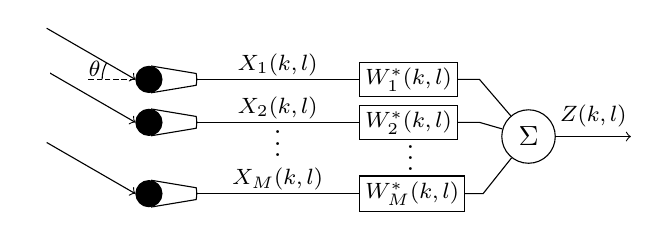
\begin{tikzpicture}
    % Adjustments
    \def\micd{.1cm}                % mic diameter
    \def\micl{.6cm}                % mic length
    \def\micw{.15cm}                % mic width
   \def\micbend{10}               % mic bottom bend
    \def\micdistance{.2cm}         % distance between microphones
    \def\filterdistance{2.5cm}     % distance between microphone and filter
    \def\filteroutline{.9cm}       % length of line which gets out of filter
    \def\sumdistance{1.5cm}        % distance of sum node to the filter
    \def\sumoutline{1cm}           % length of line which gets out of sum
    \def\headdistance{2cm}         % distance between microphone and head

    % Styles
    \tikzset{%
      mic head/.style={fill=black,draw=black,circle,minimum size=\micd},
      filter/.style={draw,minimum width=1.1cm,inner sep=2pt},
      sum/.style={draw,circle},
      xlabel/.style={inner sep=1pt,above,midway},
      sumlabel/.style={xlabel},
      hlabel/.style={xlabel,sloped,pos=.7},
      head/.style={font=\Large}
    }

    % Draw Microphones
    \begin{scope}[start chain=going below,every node/.style={on chain},node distance=\micdistance]
      \node[mic head] (mic1) {};
      \node[mic head] (mic2) {};
      \node[mic head,yshift=-1.8*\micdistance] (mic3) {};
    \end{scope}
    %\node[yshift=3pt] at ($(mic2)!.5!(mic3)$) {$\vdots$};

    \foreach \m in {1,2,3} {%
      \coordinate (m1) at ($(mic\m)+(\micl,\micw/2)$);
      \coordinate (m2) at ($(mic\m)+(\micl,-\micw/2)$);
      \draw (tangent cs:node=mic\m,point={(m1)},solution=1) -- (m1) to[bend left=\micbend] (m2) -- (tangent cs:node=mic\m,point={(m2)},solution=2);
    }

    % Draw Filter
    \foreach \m/\i in {1/1,2/2,3/M} {%
      \node[filter,right=\filterdistance of mic\m] (filter\m) {\footnotesize $W^{*}_{\i}(k,l)$};
      \draw ($(mic\m)+(\micl,0)$) to node[xlabel] (x\m) {\footnotesize $X_{\i}(k,l)$} (filter\m);
    }
    \node[yshift=3pt] at ($(filter2)!.5!(filter3)$) {$\vdots$};
    \node[yshift=3pt] at ($(x2)!.5!(x3)$) {$\vdots$};
    % Sum Node
    \node[sum] (sum) at ($(filter1)!.5!(filter3)+(\sumdistance,0)$) {$\Sigma$};
    \draw[->] (sum) -- node[above] {\footnotesize $Z(k,l)$} ++(1.3,0);
    % Connect filter with sum
    \foreach \m in {1,2,3} {%
      \draw (filter\m) -- ++(\filteroutline,0) -- (sum);
    }

    % Connect head with mics
    \foreach \m/\i in {1/1,2/2,3/M} {%
      \draw[<-] (mic\m.west) -- ++(150:1.3cm) coordinate (c\m);
%      \draw[->] (head) --  (mic\m);
    }
    % Head
    \node[head,left] (head) at (c2) {\PHtattooedHead};
    \node[fill=white,minimum width=4.8pt,minimum height=5.7pt,inner sep=0pt] at ($(head.center)+(2.3pt,-2.5pt)$) {};
%    \node at ($(head.center)+(0.0pt,-20.5pt)$) {\footnotesize $S(k,l)$};

%    \draw[dash pattern=on 2pt off 1pt,shorten <=-10pt,shorten >=-10pt] (mic1.north) -- (mic3.south);

%    Radius
    \draw ($(mic1.west)+(150:12pt)$) arc [start angle=150,end angle=180,radius=12pt];
    \draw[dash pattern=on 2pt off 1pt] (mic1.west) -- ++(left:18pt) node[inner sep=1pt,anchor=south west,font=\footnotesize] {$\theta$};
  \end{tikzpicture}
  \caption{Acoustic system configuration.}
  \label{fig: ac_sys}
\end{figure}
The $m$-th microphone signal, $m = 1, \; \ldots, \; M,$ at frequency index $k$ and frame index $l$ is given by $X_m(k,l) = X_{{\rm{d}},m}(k,l) + X_{{\rm{r}},m}(k,l)$, where $X_{{\rm{d}},m}(k,l)$ denotes the direct and early reverberant speech component and $X_{{\rm{r}},m}(k,l)$ denotes the late reverberant speech component at the $m$-th microphone.
In vector notation, the $M$-dimensional vector of the received signals $\mathbf{x}(k,l)$ can be written as 
\begin{equation}
\mathbf{x}(k,l) = \mathbf{x}_{\rm{d}}(k,l) + \mathbf{x}_{\rm{r}}(k,l),
\end{equation} 
with $\mathbf{x}(k,l) = [X_1(k,l) \; X_2(k,l) \; \ldots \; X_M(k,l)]^T$ and $\mathbf{x}_{\rm d}(k,l)$ and $\mathbf{x}_{\rm r}(k,l)$ similarly defined.
Modeling the speech source as a single point-source, the vector $\mathbf{x}_{\rm d}(k,l)$ can be expressed as
\begin{equation}
\label{eq: direct}
\mathbf{x}_{\rm d}(k,l) = S(k,l)\mathbf{d}(k),
\end{equation}
with $S(k,l)$ the target signal (i.e., direct and early reverberant speech component) as received by a reference microphone and $\mathbf{d}(k) = [D_1(k) \; D_2(k) \; \ldots \; D_M(k)]^T$ the vector of RETFs of the target signal from the reference microphone to all microphones.
The target signal is often defined as the direct speech component only, such that the vector $\mathbf{d}(k)$ can be computed based on the DOA $\theta$ of the speech source and the geometry of the microphone array~\cite{Braun_EUSIPCO_2013,Kuklasinski_EUSIPCO_2014g,Kuklasinksi_ICASSP_2015,Braun_EURASIP_2015,Schwartz_WASPAA_2015,Schwartz_ICASSP_2016,Kuklasinski_ITASLP_2016,kuklasinski_AES_2016}. 
The PSD matrix of $\mathbf{x}(k,l)$ is defined as
\begin{equation}
\mathbf{R}_{\mathbf{x}}(k,l) = {\cal{E}} \{ \mathbf{x}(k,l) \mathbf{x}^H(k,l)\}, 
%\mathbf{R}_{\mathbf{x}_{{\rm d}}}(k,l) &= {\cal{E}} \{ \mathbf{x}_{\rm d}(k,l) \mathbf{x}^H_{\rm d}(k,l)\}, \\
%\mathbf{R}_{\mathbf{x}_{{\rm r}}}(k,l) &= {\cal{E}} \{ \mathbf{x}_{\rm r}(k,l) \mathbf{x}^H_{\rm r}(k,l)\}, 
\end{equation}
where ${\cal{E}}$ denotes the expected value operator.
Assuming that $\mathbf{x}_{\rm d}(k,l)$ and $\mathbf{x}_{\rm r}(k,l)$ are uncorrelated, the PSD matrix $\mathbf{R}_{\mathbf{x}}(k,l)$ can be written as
\begin{align}
\label{eq: xcorr}
\mathbf{R}_{\mathbf{x}}(k,l) &= \mathbf{R}_{{\mathbf{x}}_{\rm d}}(k,l) + \mathbf{R}_{{\mathbf{x}}_{\rm r}}(k,l),
\end{align}
with $\mathbf{R}_{{\mathbf{x}}_{\rm d}}(k,l) = {\cal{E}} \{ \mathbf{x}_{\rm d}(k,l) \mathbf{x}^H_{\rm d}(k,l)\}$ the PSD matrix of $\mathbf{x}_{\rm d}(k,l)$ and $\mathbf{R}_{\mathbf{x}_{{\rm r}}}(k,l) = {\cal{E}} \{ \mathbf{x}_{\rm r}(k,l) \mathbf{x}^H_{\rm r}(k,l)\}$ the PSD matrix of $\mathbf{x}_{\rm r}(k,l)$.
Using~(\ref{eq: direct}), the matrix $\mathbf{R}_{\mathbf{x}_{{\rm d}}}(k,l)$ can be expressed as
\begin{equation}
\label{eq: corr_dir}
\mathbf{R}_{\mathbf{x}_{{\rm d}}}(k,l) = \Phi_{\rm s}(k,l) \mathbf{d}(k) \mathbf{d}^H(k),
\end{equation}
where $\Phi_{\rm s}(k,l)$ is the PSD of the target signal, i.e., $\Phi_{\rm s}(k,l) = {\cal{E}}\{|S(k,l)|^2\}$.
The matrix $\mathbf{R}_{\mathbf{x}_{{\rm r}}}(k,l)$ may be written as
\begin{equation}
\label{eq: corr_rev}
\mathbf{R}_{{\mathbf{x}}_{\rm r}}(k,l) = \Phi_{\rm r}(k,l){\boldsymbol{\Gamma}}(k),
\end{equation}
where $\Phi_{\rm r}(k,l)$ is the PSD of the late reverberant speech component at the reference microphone and ${\boldsymbol{\Gamma}}(k)$ denotes the time-invariant spatial coherence matrix of the late reverberation normalized by $\Phi_{\rm r}(k,l)$~\cite{Braun_EUSIPCO_2013,Kuklasinski_EUSIPCO_2014g,Kuklasinksi_ICASSP_2015,Braun_EURASIP_2015,Schwartz_WASPAA_2015,Schwartz_ICASSP_2016,Kuklasinski_ITASLP_2016,kuklasinski_AES_2016}.
Modeling the late reverberation as an isotropic sound field, ${\boldsymbol{\Gamma}}(k)$ can be analytically computed given the geometry of the microphone array~\cite{Braun_EUSIPCO_2013,Braun_EURASIP_2015,Schwartz_WASPAA_2015,Schwartz_ICASSP_2016}.
Defining the filter coefficients vector $\mathbf{w}(k,l) = [W_1(k,l) \; W_2(k,l) \; \ldots \; W_M(k,l)]^T$, the output signal $Z(k,l)$ of the speech enhancement system is given by
\begin{equation}
Z(k,l) = \mathbf{w}^H(k,l)\mathbf{x}_{\rm d}(k,l) + \mathbf{w}^H(k,l)\mathbf{x}_{\rm r}(k,l).
\end{equation}
Speech dereverberation techniques design the filter $\mathbf{w}(k,l)$ such that the output signal $Z(k,l)$ resembles the target signal $S(k,l)$.
Many such techniques require an estimate of the late reverberant PSD $\Phi_{\rm r}(k,l)$, e.g.,~\cite{Braun_EUSIPCO_2013,Kuklasinski_EUSIPCO_2014g,OSchwartz_ITASLP_2015}.
State-of-the-art multi-channel late reverberant PSD estimators~\cite{Braun_EUSIPCO_2013,Kuklasinski_EUSIPCO_2014g,Braun_EURASIP_2015,Schwartz_WASPAA_2015,Schwartz_ICASSP_2016,Kuklasinski_ITASLP_2016} rely on knowledge of the vector $\mathbf{d}(k)$, which may be difficult to estimate accurately.
%As shown in~\cite{Braun_EURASIP_2015,ASchwarz_ITASLP_2015, kuklasinski_AES_2016}, estimation errors in $\mathbf{d}(k)$ degrade the PSD estimation accuracy, degrading as a result the dereverberation performance of the used speech enhancement system.
In the following, a novel late reverberant PSD estimator is proposed which does not require knowledge of $\mathbf{d}(k)$.
% While the RTF vector $\mathbf{d}$ and the coherence matrix $\boldsymbol{\Gamma}$ are time-invariant and assumed to be known, the PSDs $\Phi_{\rm s}(l)$ and $\Phi_{\rm r}(l)$ are time-varying and need to be estimated.
For conciseness the frequency index $k$ is omitted in the remainder of this paper.

It should be noted that for the sake of simplicity and to be able to compare the proposed estimator to the ML estimator in~\cite{Kuklasinski_EUSIPCO_2014g}, a noise-free scenario is assumed in this paper. 
Nevertheless, the late reverberant PSD estimator proposed in Section~\ref{sec: evd} can also be used in a noisy scenario, as long as an estimate of $\mathbf{R}_{\mathbf{x}}(l)$ can be obtained by e.g., subtracting the noise component PSD matrix from the noisy signal PSD matrix.


% \section{Multi-channel Wiener filter for \\ Speech Dereverberation}
% \label{sec: mwf}
% Since the PSD estimators considered in this paper are used in a MWF in Section~\ref{sec: exp}, in this section the MWF for speech dereverberation is briefly reviewed.
% The MWF aims at dereverberation by minimizing the mean-square error between the output signal and the target signal~\cite{Braun_EUSIPCO_2013,Kuklasinski_EUSIPCO_2014g}.

% The MWF cost function can then be written as
% \begin{equation}
% \label{eq: mwf_cost}
% J_{_{\text{MWF}}}(l) =  {\cal{E}}  \{|\mathbf{w}^H(l)\mathbf{x}_{\rm d}(l) - S(l) |^2 \} + {\cal{E}} \{|\mathbf{w}^H(l)\mathbf{x}_{\rm r}(l) |^2 \}.
% \end{equation}
% The minimization of~(\ref{eq: mwf_cost}) yields
% \begin{align}
% \label{eq: mwf}
% \mathbf{w}_{_{\text{MWF}}}(l) &= [\mathbf{R}_{\mathbf{x}_{{\rm d}}}(l) + \mathbf{R}_{\mathbf{x}_{{\rm r}}}(l)]^{-1} { \cal{E} } \{ \mathbf{x}_{{\rm d}}(l) S^*(l) \} \\
% \label{eq: mwf_2}
%  &= [\Phi_{\rm s}(l)\mathbf{d}\mathbf{d}^H + \Phi_{\rm r}(l)\boldsymbol{\Gamma}]^{-1}\Phi_{\rm s}(l)\mathbf{d}.
% \end{align}
% It is well known that the MWF can be decomposed into an MVDR beamformer $\mathbf{w}_{_{\text{MVDR}}}$ and a single-channel Wiener postfilter $G(l)$ applied to the MVDR output~\cite{Simmer_book_2001}, i.e.,
% \begin{equation}
% \label{eq: decomp}
% \mathbf{w}_{_{\text{MWF}}}(l) = \underbrace{\frac{\boldsymbol{\Gamma}^{-1}\mathbf{d}}{\mathbf{d}^H\boldsymbol{\Gamma}^{-1}\mathbf{d}}}_{\mathbf{w}_{_{\text{MVDR}}}} \underbrace{\frac{\Phi_{\rm s_o}(l)}{\Phi_{\rm s_o}(l) + \Phi_{\rm r_o}(l)}}_{G(l)},
% \end{equation}
% with $\Phi_{\rm s_o}(l)$ and $\Phi_{\rm r_o}(l)$ the PSDs of the target signal and late reverberant speech component at the output of the MVDR beamformer given by
% \begin{equation}
% \label{eq: out_pow}
% \Phi_{\rm s_o}(l) = \Phi_{\rm s}(l), \; \; \; \; \Phi_{\rm r_o}(l) = \frac{\Phi_{\rm r}(l)}{\mathbf{d}^H\boldsymbol{\Gamma}^{-1}\mathbf{d}}.
% \end{equation}
% While the PSD of the target signal is not changed by the MVDR beamformer, the PSD of the late reverberant speech component needs to be corrected by the beamformer suppression factor.
% The MVDR beamformer $\mathbf{w}_{_{\text{MVDR}}}$ in~(\ref{eq: decomp}) is time-invariant and depends on the normalized coherence matrix $\boldsymbol{\Gamma}$ and the vector $\mathbf{d}$.
% Assuming that $\boldsymbol{\Gamma}$ and $\mathbf{d}$ are known, the MVDR beamformer can be calculated beforehand.
% On the other hand, the single-channel Wiener filter $G(l)$ depends on the time-varying PSDs $\Phi_{\rm s}(l)$ and $\Phi_{\rm r}(l)$ (cf.~(\ref{eq: decomp}) and~(\ref{eq: out_pow})), which need to be estimated.
% In this paper, we propose a novel method to estimate the late reverberant PSD $\Phi_{\rm r}(l)$.

\section{Late Reverberant \\ Power Spectral Density Estimator}
In this section the ML estimator proposed in~\cite{Kuklasinski_EUSIPCO_2014g} is briefly reviewed and a novel eigenvalue decomposition~(EVD)-based estimator is proposed.
%In addition, analytical insights on the relation between these two estimators are provided.

\subsection{Maximum likelihood estimator}
In order to derive the ML estimator in~\cite{Kuklasinski_EUSIPCO_2014g}, the spectral coefficients of the direct and late reverberant speech  components are assumed to be circularly-symmetric complex Gaussian distributed.
These distributions are then used to construct and maximize a likelihood function, resulting in the PSD estimates
\begin{subequations}
\label{eq: psd_ml}
\begin{align}
\label{eq: phir_ml}
\hat{\Phi}_{\rm r}^{\rm ml}(l) & = \frac{1}{M-1} {\rm tr} \left\{  \left( \mathbf{I} - \mathbf{d} \frac{\mathbf{d}^{H}\boldsymbol{\Gamma}^{-1}}{\mathbf{d}^H\boldsymbol{\Gamma}^{-1}\mathbf{d}} \right) \mathbf{R}_{\mathbf{x}}(l)\boldsymbol{\Gamma}^{-1}\right\}, \\
\hat{\Phi}_{\rm s}^{\rm ml}(l) & = \frac{\mathbf{d}^{H}\boldsymbol{\Gamma}^{-1}}{\mathbf{d}^H\boldsymbol{\Gamma}^{-1}\mathbf{d}} \left[\mathbf{R}_{\mathbf{x}}(l) - \hat{\Phi}_{\rm r}^{\rm ml}(l) \boldsymbol{\Gamma} \right] \frac{\boldsymbol{\Gamma}^{-1}\mathbf{d}}{\mathbf{d}^H\boldsymbol{\Gamma}^{-1}\mathbf{d}},
\end{align}
\end{subequations}
where ${\rm tr}\{ \cdot \}$ denotes the matrix trace operator.
The ML late reverberant PSD estimate in~(\ref{eq: phir_ml}) requires an estimate of the PSD matrix $\mathbf{R}_{\mathbf{x}}(l)$, normalized coherence matrix $\boldsymbol{\Gamma}$, and vector $\mathbf{d}$.
While $\mathbf{R}_{\mathbf{x}}(l)$ can be estimated from the received signal $\mathbf{x}(l)$ and $\boldsymbol{\Gamma}$ can be constructed assuming a reasonable sound field model for the late reverberation, accurately estimating the vector $\mathbf{d}$ may be difficult.
As is experimentally validated in~\cite{kuklasinski_AES_2016}, estimation errors in the vector $\mathbf{d}$ degrade the PSD estimation accuracy of the ML estimator in~(\ref{eq: phir_ml}), yielding as a result a degradation in the dereverberation performance of the used speech enhancement system.

\subsection{Eigenvalue decomposition-based estimator}
\label{sec: evd}
Aiming to remove the dependency of the PSD estimate on the vector $\mathbf{d}$, in the following we propose to estimate the late reverberant PSD using the eigenvalues of the prewhitened received signal PSD matrix $\mathbf{R}_{\mathbf{x}}(l)\boldsymbol{\Gamma}^{-1}$.
Let us first consider the EVD of $\mathbf{R}_{{\mathbf{x}}_{\rm d}}(l)\boldsymbol{\Gamma}^{-1}$, i.e.,
\begin{equation}
\label{eq: evd_rxd}
\mathbf{R}_{{\mathbf{x}}_{\rm d}}(l)\boldsymbol{\Gamma}^{-1} = \mathbf{U} \mathbf{S}_{{\mathbf{x}}_{\rm d}}(l)\mathbf{U}^{-1},
\end{equation}
with $\mathbf{U}$ being an $M \times M$-dimensional matrix of eigenvectors and $\mathbf{S}_{{\mathbf{x}}_{\rm d}}(l)$ being the $M \times M$-dimensional diagonal matrix of eigenvalues.
Since the matrix $\mathbf{R}_{\mathbf{x}_{\rm d}}(l)\boldsymbol{\Gamma}^{-1}$ is a rank-1 matrix, $\mathbf{S}_{{\mathbf{x}}_{\rm d}}(l)$ has only one non-zero eigenvalue $\sigma(l)$, i.e., 
\begin{equation}
\mathbf{S}_{{\mathbf{x}}_{\rm d}}(l) = {\rm diag} \{[\sigma(l) \; \; 0 \; \; \ldots \;\; 0]^T \}.
\end{equation}
Using~(\ref{eq: xcorr}) and~(\ref{eq: evd_rxd}), the EVD of the prewhitened received signal PSD matrix $\mathbf{R}_{\mathbf{x}}(l)\boldsymbol{\Gamma}^{-1}$ can be written as
\begin{subequations}
\label{eq: evd_rx}
\begin{align}
\mathbf{R}_{\mathbf{x}}(l)\boldsymbol{\Gamma}^{-1}  & = \mathbf{U} \mathbf{S}_{{\mathbf{x}}_{\rm d}}(l) \mathbf{U}^{-1} + \Phi_{\rm r}(l)\mathbf{I} \\
& = \mathbf{U} [\underbrace{\mathbf{S}_{{\mathbf{x}}_{\rm d}}(l) + \Phi_{\rm r}(l)\mathbf{I}}_{\mathbf{S}_{\mathbf{x}}(l)}]\mathbf{U}^{-1},
\end{align}
\end{subequations}
with $\mathbf{S}_{\mathbf{x}}(l)$ the $M \times M$-dimensional diagonal matrix of eigenvalues given by
\begin{equation}
\label{eq: tildes}
\mathbf{S}_{\mathbf{x}}(l) = {\rm diag} \{[\sigma(l) + \Phi_{\rm r}(l) \; \; \Phi_{\rm r}(l) \;\; \ldots \;\; \Phi_{\rm r}(l)]^T \}.
\end{equation}
Based on~(\ref{eq: evd_rx}) and~(\ref{eq: tildes}), we propose to estimate the late reverberant PSD using any of the eigenvalues of the prewhitened received signal PSD matrix $\mathbf{R}_{\mathbf{x}}(l)\boldsymbol{\Gamma}^{-1}$, i.e.,
\begin{subequations}
\label{eq: phir_evd}
\begin{align}
\label{eq: phir_evds}
\hat{\Phi}^{\rm evd}_{\rm r}(l) & = \lambda_2\{\mathbf{R}_{\mathbf{x}}(l)\boldsymbol{\Gamma}^{-1}\} = \cdots = \lambda_M\{\mathbf{R}_{\mathbf{x}}(l)\boldsymbol{\Gamma}^{-1}\} \\
\label{eq: evd_tr}
& =\frac{1}{M-1} \left( {\rm tr} \left\{ \mathbf{R}_{\mathbf{x}}(l)\boldsymbol{\Gamma}^{-1} \right\} - \lambda_1\left\{\mathbf{R}_{\mathbf{x}}(l)\boldsymbol{\Gamma}^{-1}\right\}\right), 
\end{align}
\end{subequations}
where $\lambda_i\{ \cdot \}$ denotes the $i$-th eigenvalue.
The equality in~(\ref{eq: evd_tr}) is derived using the fact that the trace of a matrix is equal to the sum of its eigenvalues. 
Using $\hat{\Phi}^{\rm evd}_{{\rm r}}(l)$, the target signal PSD $\Phi^{\rm evd}_{{\rm s}}(l)$ is estimated using the decision directed approach~\cite{Ephraim_ITASSP_1984}.

% \begin{equation}
% \label{eq: phis_evd}
% \hat{\Phi}_{\rm s}^{\rm evd}(l)  = \mathbf{w}^H_{_{\text{MVDR}}} \left[\mathbf{R}_{\mathbf{x}}(l) - \hat{\Phi}_{\rm r}^{\rm evd}(l) \boldsymbol{\Gamma} \right] \mathbf{w}_{_{\text{MVDR}}}.
% \end{equation}
While the ML estimate in~(\ref{eq: phir_ml}) requires knowledge of $\mathbf{R}_{\mathbf{x}}(l)$, $\boldsymbol{\Gamma}$, and $\mathbf{d}$, the proposed EVD-based estimate in~(\ref{eq: phir_evd}) requires only knowledge of $\mathbf{R}_{\mathbf{x}}(l)$ and $\boldsymbol{\Gamma}$.
Clearly, if $\mathbf{R}_{\mathbf{x}}(l)$ and $\boldsymbol{\Gamma}$ are perfectly known, the EVD-based PSD estimate in~(\ref{eq: phir_evd}) is equal to the true late reverberant PSD, i.e., $\hat{\Phi}^{\rm evd}_{\rm r}(l) = \Phi_{\rm r}(l)$.
In practice however, the available PSD matrix $\tilde{\mathbf{R}}_{\mathbf{x}}(l)$ and normalized coherence matrix $\tilde{\boldsymbol{\Gamma}}$ might differ from the true quantities $\mathbf{R}_{\mathbf{x}}(l)$ and $\boldsymbol{\Gamma}$. 
For $\tilde{\mathbf{R}}_{\mathbf{x}}(l) \neq \mathbf{R}_{\mathbf{x}}(l)$ and $\tilde{\boldsymbol{\Gamma}} \neq \boldsymbol{\Gamma}$, the EVD of $\tilde{\mathbf{R}}_{\mathbf{x}}(l) \tilde{\boldsymbol{\Gamma}}^{-1}$ differs from the desired EVD in~(\ref{eq: evd_rx}).
Furthermore, the prewhitening of $\tilde{\mathbf{R}}_{\mathbf{x}}(l)$ using $\tilde{\boldsymbol{\Gamma}}^{-1}$ fails, and hence, the last $M-1$ eigenvalues of $\tilde{\mathbf{R}}_{\mathbf{x}}(l)\tilde{\boldsymbol{\Gamma}}^{-1}$ are not equal, i.e.,
\begin{equation}
\lambda_2\{\tilde{\mathbf{R}}_{\mathbf{x}}(l) \tilde{\boldsymbol{\Gamma}}^{-1}\} \neq \lambda_3\{\tilde{\mathbf{R}}_{\mathbf{x}}(l) \tilde{\boldsymbol{\Gamma}}^{-1}\} \neq \ldots \neq \lambda_M\{\tilde{\mathbf{R}}_{\mathbf{x}}(l) \tilde{\boldsymbol{\Gamma}}^{-1}\}.
\end{equation}
As a result, different late reverberant PSD estimates are obtained depending on the eigenvalue used for the estimation.
In the remainder of this work, $\hat{\Phi}^{\rm evd}_{{\rm r},i}(l)$ will be used to denote the late reverberant PSD estimate when using the $i$-th eigenvalue of $\tilde{\mathbf{R}}_{\mathbf{x}}(l)\tilde{\boldsymbol{\Gamma}}^{-1}$, i.e.,
\begin{equation}
\label{eq: psd_evd_mis1}
\hat{\Phi}_{{\rm r},i}^{\rm evd}(l) = \lambda_i\left\{ \tilde{\mathbf{R}}_{\mathbf{x}}(l) \tilde{\boldsymbol{\Gamma}}^{-1} \right\}, \; \; \; \; i = 2, \ldots, M.
\end{equation}
Furthermore, $\hat{\Phi}^{\rm evd}_{{\rm r,tr}}(l)$ will be used to denote the late reverberant PSD estimate when using the trace and the first eigenvalue of $\tilde{\mathbf{R}}_{\mathbf{x}}(l) \tilde{\boldsymbol{\Gamma}}^{-1}$, i.e.,
\begin{equation}
\label{eq: psd_evd_mis2}
\hat{\Phi}^{\rm evd}_{{\rm r,tr}}(l) = \frac{1}{M-1}\left( {\rm tr} \left\{ \tilde{\mathbf{R}}_{\mathbf{x}}(l) \tilde{\boldsymbol{\Gamma}}^{-1} \right\} - \lambda_1\left\{\tilde{\mathbf{R}}_{\mathbf{x}}(l)\tilde{\boldsymbol{\Gamma}}^{-1}\right\}\right).
\end{equation}
In Section~\ref{sec: exp} the performance of the PSD estimate in~(\ref{eq: psd_evd_mis1}) with $i = 2$ as well as of the PSD estimate in~(\ref{eq: psd_evd_mis2}) is investigated.

% % In practice however, the available RTF vector $\tilde{\mathbf{d}}$ and coherence matrix $\tilde{\boldsymbol{\Gamma}}$ might differ from the true RTF vector $\mathbf{d}$ and true coherence matrix $\boldsymbol{\Gamma}$.
% % In the presence of RTF vector or coherence matrix mismatches, the EVD- and ML-based estimates are not equaivalent and the equalities in~(\ref{eq: equiv})-(\ref{eq: der5a}) do not hold.
% % In the presence of RTF vector mismatches, i.e.,  $\tilde{\mathbf{d}}\neq \mathbf{d}$, the EVD-based estimate in~(\ref{eq: phir_evd}) still yields the true reverberation PSD (since it is independent of the RTF vector) whereas the ML-based estimate in~(\ref{eq: der3}) results in an erronous reverberation PSD estimate~(since it explicitly relies on the RTF vector).

\section{Experimental Results}
\label{sec: exp}
In this section the dereverberation performance of a MWF using the considered ML and EVD-based PSD estimators is compared when the DOA is perfectly estimated as well as in the presence of DOA estimation errors.
As in e.g.,~\cite{Braun_EUSIPCO_2013,Kuklasinski_EUSIPCO_2014g}, the MWF is implemented as an MVDR beamformer ${\mathbf{w}_{_{\text{MVDR}}}}$ followed by a single-channel Wiener postfilter $G(l)$ applied to the MVDR output, i.e.,
% The minimization of~(\ref{eq: mwf_cost}) yields
% \begin{align}
% \label{eq: mwf}
% \mathbf{w}_{_{\text{MWF}}}(l) &= [\mathbf{R}_{\mathbf{x}_{{\rm d}}}(l) + \mathbf{R}_{\mathbf{x}_{{\rm r}}}(l)]^{-1} { \cal{E} } \{ \mathbf{x}_{{\rm d}}(l) S^*(l) \} \\
% \label{eq: mwf_2}
%  &= [\Phi_{\rm s}(l)\mathbf{d}\mathbf{d}^H + \Phi_{\rm r}(l)\boldsymbol{\Gamma}]^{-1}\Phi_{\rm s}(l)\mathbf{d}.
% \end{align}
\begin{equation}
\label{eq: decomp}
\mathbf{w}_{_{\text{MWF}}}(l) = \underbrace{\frac{\tilde{\boldsymbol{{\Gamma}}}^{-1}\mathbf{d}}{\mathbf{d}^H\tilde{\boldsymbol{{\Gamma}}}^{-1}\mathbf{d}}}_{\mathbf{w}_{_{\text{MVDR}}}} \underbrace{\frac{\Phi_{\rm s_o}(l)}{\Phi_{\rm s_o}(l) + \Phi_{\rm r_o}(l)}}_{G(l)},
\end{equation}
with $\Phi_{\rm s_o}(l)$ and $\Phi_{\rm r_o}(l)$ the PSDs of the target signal and late reverberant speech component at the output of the MVDR beamformer given by
\begin{equation}
\label{eq: out_pow}
\Phi_{\rm s_o}(l) = \Phi_{\rm s}(l), \; \; \; \; \Phi_{\rm r_o}(l) = \frac{\Phi_{\rm r}(l)}{\mathbf{d}^H\tilde{\boldsymbol{\Gamma}}^{-1}\mathbf{d}}.
\end{equation}
While the PSD of the target signal is not changed by the MVDR beamformer, the PSD of the late reverberant speech component needs to be corrected by the beamformer suppression factor.
The MVDR beamformer $\mathbf{w}_{_{\text{MVDR}}}$ in~(\ref{eq: decomp}) is time-invariant and depends on the available normalized coherence matrix $\tilde{\boldsymbol{\Gamma}}$ and vector $\mathbf{d}$.
On the other hand, the single-channel Wiener filter $G(l)$ depends on the time-varying PSDs $\Phi_{\rm s}(l)$ and $\Phi_{\rm r}(l)$, cf.~(\ref{eq: decomp}) and~(\ref{eq: out_pow}), which are estimated using the considered ML and EVD-based estimators.
It should be noted that independently of the PSD estimator used, the MWF implemented according to~(\ref{eq: decomp}) is sensitive to errors in the vector $\mathbf{d}$ due to the sensitivity of the MVDR beamformer to errors in $\mathbf{d}$.
However, as shown in Section~\ref{sec: exp2}, a significantly higher sensitivity of the MWF is observed when also the used PSD estimator is affected by errors in the vector $\mathbf{d}$.

\subsection{Setup}
We consider two multi-channel acoustic systems with $M \in \{2, 3, 4 \}$ microphones and a single speech source located at an angle $\theta = 45^{\circ}$ and at a distance of $2$~m from the microphone array.
The first acoustic system consists of a linear microphone array with an inter-sensor distance of $8$~cm placed in a room with reverberation time $T_{60} \approx 610$~ms~\cite{hadad_IWAENC_2014}.
The second acoustic system consists of a circular microphone array with a radius of $10$~cm placed in a room with reverberation time $T_{60} \approx 730$~ms~\cite{REVERB2016}.
The sampling frequency is $f_s = 16$ kHz and the received reverberant signals are generated by convolving clean speech signals from the HINT database~\cite{Nilsson_JASA_1994} with the measured RIRs. 

The signals are processed using a weighted overlap-add framework with a frame size of $1024$ samples and an overlap of $75 \%$ between successive frames. 
The first microphone is arbitrarily selected as the reference microphone.
In order to implement the MWF, the vector $\mathbf{d}$, the normalized coherence matrix $\tilde{\boldsymbol{\Gamma}}$, and the received signal PSD matrix $\tilde{\mathbf{R}}_{\mathbf{x}}(l)$ are required.
As in e.g.,~\cite{Kuklasinski_EUSIPCO_2014g,Kuklasinksi_ICASSP_2015,kuklasinski_AES_2016}, the vector $\mathbf{d}$ is computed from the respective RIRs truncated to the part containing only the direct path response.
As in e.g.,~\cite{Braun_EUSIPCO_2013,Braun_EURASIP_2015}, the normalized coherence matrix $\tilde{\boldsymbol{\Gamma}}$ is computed assuming a spherically isotropic sound field. %, resulting in the well-known superdirective beamformer~\cite{Simmer_book2_2001}.
%Since superdirective beamformers are sensitive to uncorrelated noise~\cite{Simmer_book2_2001}, a white noise gain constraint of $-10$ dB is imposed.
In none of the considered acoustic systems the late reverberation is truly isotropic, resulting in a mismatch between the available coherence matrix $\tilde{\boldsymbol{\Gamma}}$ and the true coherence matrix $\boldsymbol{\Gamma}$.
The received signal PSD matrix $\tilde{\mathbf{R}}_{\mathbf{x}}(l)$ is estimated from $\mathbf{x}(l)$ using recursive averaging with a time constant of $40$ ms.
The minimum gain of the single-channel Wiener postfilter is set to $-20$ dB.

The performance is evaluated in terms of the improvement in frequency-weighted segmental signal-to-noise-ratio ($\Delta$fwSSNR) \cite{Hu_ITASLP_2008} and the improvement in cepstral distance~($\Delta$CD)~\cite{Quackenbush_book} between the output speech signal and the reference microphone signal.
The fwSSNR and CD measures are intrusive measures comparing the output signal to a reference signal. 
The reference signal used in this paper is the anechoic speech signal.
It should be noted that a positive $\Delta$fwSSNR and a negative $\Delta$CD indicate a performance improvement.

The performance of the MVDR beamformer in~(\ref{eq: decomp}) and of the MWF implemented according to~(\ref{eq: decomp}) using the ML and EVD-based PSD estimates is investigated for 
\begin{itemize}
\item[i)] both acoustic systems with different number of microphones $M \in \{2, 3, 4 \}$ and assuming {\emph{the DOA is perfectly estimated}}, i.e., the vector $\mathbf{d}$ is computed from the truncated RIRs corresponding to the true DOA $\theta = 45^{\circ}$ (Section~\ref{sec: exp1}), 
\item[ii)] the first acoustic system with $M = 4$ microphones and assuming {\emph{DOA estimation errors}}, i.e., the vector $\mathbf{d}$ is computed from the truncated RIRs corresponding to several erroneous DOAs $\hat{\theta} \in \{-90, -75, \ldots, 90 \}$. 
In other words, the actual source position is always at $\theta = 45^{\circ}$, but the vector $\mathbf{d}$ is computed using different DOAs $\hat{\theta}$ (Section~\ref{sec: exp2}).
\end{itemize}

\subsection{Performance when the DOA is perfectly estimated}
\label{sec: exp1}
Fig.~\ref{fig: perfect} depicts the $\Delta$fwSSNR and $\Delta$CD obtained for the MVDR beamformer and the MWF using late reverberant PSD estimates $\hat{\Phi}^{\rm ml}_{\rm r}(l)$, $\hat{\Phi}^{\rm evd}_{\rm r,2}(l)$, and $\hat{\Phi}^{\rm evd}_{\rm r,tr}(l)$.
As expected, it can be observed that the MWF using any of the considered PSD estimates improves the performance in comparison to the MVDR beamformer.
In addition, it can be observed that the performance of the MVDR beamformer and of the MWF using any of the considered PSD estimates increases with increasing number of microphones (except for the $\Delta$CD obtained when using the MWF with $\hat{\Phi}^{\rm evd}_{\rm r,2}(l)$ being slightly worse for $M = 4$ than for $M = 3$).
For both acoustic systems and all considered configurations, the proposed EVD-based PSD estimate $\hat{\Phi}^{\rm evd}_{\rm r,tr}(l)$ typically yields the best performance, always outperforming the ML estimate $\hat{\Phi}^{\rm ml}_{\rm r}(l)$.
Furthermore, the EVD-based estimate $\hat{\Phi}^{\rm evd}_{\rm r,2}(l)$ also outperforms the ML estimate $\hat{\Phi}^{\rm ml}_{\rm r}(l)$ in terms of the $\Delta$fwSSNR, while a lower performance is obtained in terms of the $\Delta$CD for $M = 4$.
It should be noted that for $M=2$, $\hat{\Phi}^{\rm evd}_{\rm r,2}(l) = \hat{\Phi}^{\rm evd}_{\rm r,tr}(l)$, cf.~(\ref{eq: psd_evd_mis1}) and~(\ref{eq: psd_evd_mis2}), and hence the performance when using these EVD-based PSD estimates is the same.

In summary, it can be said that among the proposed EVD-based PSD estimates $\hat{\Phi}^{\rm evd}_{\rm r,2}(l)$ and $\hat{\Phi}^{\rm evd}_{\rm r,tr}(l)$, using $\hat{\Phi}^{\rm evd}_{\rm r,tr}(l)$ in a MWF generally yields a better performance.
In addition, the proposed EVD-based PSD estimate $\hat{\Phi}^{\rm evd}_{\rm r,tr}(l)$ yields a better performance than the ML estimate $\hat{\Phi}^{\rm ml}_{\rm r}(l)$.

\begin{figure}[t!]

% This file was created by matlab2tikz v0.4.0.
% Copyright (c) 2008--2013, Nico Schlömer <nico.schloemer@gmail.com>
% All rights reserved.
% 
% The latest updates can be retrieved from
%   http://www.mathworks.com/matlabcentral/fileexchange/22022-matlab2tikz
% where you can also make suggestions and rate matlab2tikz.
% 
% 
% 

% defining custom colors
\definecolor{mycolor1}{rgb}{0,0,0.5625}%
\definecolor{mycolor2}{rgb}{0,0.875,1}%
\definecolor{mycolor3}{rgb}{1,0.8125,0}%

\begin{tikzpicture}[font = \small]

\begin{axis}[%
width=0.45\figurewidth,
height=\figureheight,
area legend,
scale only axis,
xmin=0.5,
xmax=3.5,
xtick={1, 2, 3},
xticklabels = {2, 3, 4},
xlabel={$M$},
xmajorgrids,
ymin=0,
ymax=6,
ylabel={$\Delta$fwSSNR [dB]},
ylabel absolute, ylabel style={yshift=-0.9em},
ymajorgrids,
name=plot1,
x label style={at={(axis description cs:0.5,0.08)},anchor=north},
title={$T_{60} \approx 610$ ms},
legend columns = 4,
area legend,
legend style={at={([xshift=15pt,yshift=20pt] 1,1)},anchor=south},
legend image post style={xscale=0.8},
legend entries = {MVDR, $\hat{\Phi}^{\rm ml}_{\rm r}(l)$,$\hat{\Phi}^{\rm evd}_{\rm r,2}(l)$,$\hat{\Phi}^{\rm evd}_{\rm r,tr}(l)$}
]
\addplot[ybar,bar width=0.01863636363636364\figurewidth,bar shift=-0.0355\figurewidth,pattern = horizontal lines,draw=black] plot coordinates{(1,1.56276872890609)
(2,2.4054)
(3,2.97017804671462)};
%\addlegendentry{MVDR};

\addplot [
color=black,
solid,
forget plot
]
table[row sep=crcr]{
0 0\\
4 0\\
};
\addplot[ybar,bar width=0.01863636363636364\figurewidth,bar shift=-0.01227272727272727\figurewidth,pattern = north west lines,draw=black] plot coordinates{(1,3.82068119844275)
(2,4.5961)
(3,4.7564541498539)};
%\addlegendentry{$\hat{\Phi}^{\rm ml}_{\rm r}(l)$};

\addplot[ybar,bar width=0.0186363636363636364\figurewidth,bar shift=0.01227272727272727\figurewidth,pattern = crosshatch,draw=black] plot coordinates{(1,4.38159428154979)
(2,5.4455)
(3,5.42045173925162)};

%\addlegendentry{$\hat{\Phi}^{\rm evd}_{\rm r,2}(l)$};

\addplot[ybar,bar width=0.01863636363636364\figurewidth,bar shift=0.0355\figurewidth,pattern = dots,draw=black] plot coordinates{(1,4.38159428154975)
(2,5.1883)
(3,5.51200776712404)};
%\addlegendentry{$\hat{\Phi}^{\rm evd}_{\rm r,tr}(l)$};
\end{axis}

\begin{axis}[%
width=0.45\figurewidth,
height=\figureheight,
area legend,
scale only axis,
xmin=0.5,
xmax=3.5,
xtick={1, 2, 3},
xticklabels = {2, 3, 4},
xlabel={$M$},
xmajorgrids,
ymin=0,
ymax=6,
%ylabel={$\Delta\text{ fwSSNR [dB]}$},
ymajorgrids,
name=plot2,
at={($(plot1.south east)+(30,0)$)},
x label style={at={(axis description cs:0.5,0.08)},anchor=north},
%anchor=south west,
title={$T_{60} \approx 730$ ms}
]
\addplot[ybar,bar width=0.01863636363636364\figurewidth,bar shift=-0.0355\figurewidth,pattern = horizontal lines,draw=black] plot coordinates{(1,0.919802659839034)
(2,1.6075)
(3,2.003300086677)};

\addplot [
color=black,
solid,
forget plot
]
table[row sep=crcr]{
0 0\\
4 0\\
};
\addplot[ybar,bar width=0.01863636363636364\figurewidth,bar shift=-0.0127272727272727\figurewidth,draw=black,pattern = north west lines] plot coordinates{(1,2.13441211187969)
(2,2.8174)
(3,3.41616793179622)};

\addplot[ybar,bar width=0.01863636363636364\figurewidth,bar shift=0.0127272727272727\figurewidth,pattern = crosshatch,draw=black] plot coordinates{(1,2.85890761597348)
(2,3.7336)
(3,4.04789288125231)};

\addplot[ybar,bar width=0.01863636363636364\figurewidth,bar shift=0.0355\figurewidth,pattern = dots,draw=black] plot coordinates{(1,2.85890761597349)
(2,3.6125)
(3,4.18550239900989)};
\end{axis}

\begin{axis}[%
width=0.45\figurewidth,
height=\figureheight,
area legend,
scale only axis,
xmin=0.5,
xmax=3.5,
xtick={1, 2, 3},
xticklabels = {2, 3, 4},
xlabel={$M$},
xmajorgrids,
ymin=-1.5,
ymax=0,
ymajorgrids,
name=plot4,
at={($(plot2.south west)-(0,40)$)},
x label style={at={(axis description cs:0.5,0.08)},anchor=north},
anchor=north west,
]
\addplot[ybar,bar width=0.01863636363636364\figurewidth,bar shift=-0.0355\figurewidth,pattern = horizontal lines,draw=black] plot coordinates{(1,-0.331009689200296)
(2,-0.5582)
(3,-0.708431214059022)};

\addplot [
color=black,
solid,
forget plot
]
table[row sep=crcr]{
0 0\\
4 0\\
};
\addplot[ybar,bar width=0.01863636363636364\figurewidth,bar shift=-0.0127272727272727\figurewidth,pattern = north west lines,draw=black] plot coordinates{(1,-0.6790106355355)
(2,-0.9240)
(3,-1.07787280937685)};

\addplot[ybar,bar width=0.01863636363636364\figurewidth,bar shift=0.0127272727272727\figurewidth,pattern = crosshatch,draw=black] plot coordinates{(1,-0.731312594136379)
(2,-0.8483)
(3,-0.782351016709798)};

\addplot[ybar,bar width=0.01863636363636364\figurewidth,bar shift=0.0355\figurewidth,pattern = dots,draw=black] plot coordinates{(1,-0.731312594136377)
(2,-0.9750)
(3,-1.14625607409604)};
\end{axis}

\begin{axis}[%
width=0.45\figurewidth,
height=\figureheight,
area legend,
scale only axis,
xmin=0.5,
xmax=3.5,
xtick={1, 2, 3},
xticklabels = {2, 3, 4},
xlabel={$M$},
xmajorgrids,
ymin=-1.5,
ylabel={$\Delta$CD [dB]},
ylabel absolute, ylabel style={yshift=-0.9em},
ymax=0,
ymajorgrids,
name=plot3,
at={($(plot1.south west)-(0,40)$)},
x label style={at={(axis description cs:0.5,0.08)},anchor=north},
anchor=north west
]
\addplot[ybar,bar width=0.01863636363636364\figurewidth,bar shift=-0.0355\figurewidth,pattern = horizontal lines,,draw=black] plot coordinates{(1,-0.348155732776004)
(2,-0.5262)
(3,-0.639446818906877)};

\addplot [
color=black,
solid,
forget plot
]
table[row sep=crcr]{
0 0\\
4 0\\
};
\addplot[ybar,bar width=0.01863636363636364\figurewidth,bar shift=-0.0127272727272727\figurewidth,draw=black,  pattern = north west lines] plot coordinates{(1,-0.817608927542006)
(2,-0.9336)
(3,-1.01373612500695)};

\addplot[ybar,bar width=0.01863636363636364\figurewidth,bar shift=0.0127272727272727\figurewidth,pattern = crosshatch,draw=black] plot coordinates{(1,-0.925719680815751)
(2,-1.0284)
(3,-0.928233701255566)};

\addplot[ybar,bar width=0.01863636363636364\figurewidth,bar shift=0.0355\figurewidth,pattern = dots,draw=black] plot coordinates{(1,-0.925719680815749)
(2,-1.1173)
(3,-1.2072132043461)};

\end{axis}

\node[below] at ([yshift=-15pt] $(plot1.south)!.5!(plot2.south)$) {(a)};
\node[below] at ([yshift=-15pt] $(plot3.south)!.5!(plot4.south)$) {(b)};
\end{tikzpicture}%

%%% Local Variables:
%%% mode: latex
%%% TeX-master: "../Template"
%%% End:

\caption{Performance of the MVDR beamformer and the MWF using $\hat{\Phi}^{\rm ml}_{\rm r}(l)$, $\hat{\Phi}^{\rm evd}_{\rm r, 2}(l)$, and $\hat{\Phi}^{\rm evd}_{\rm r, tr}(l)$ when the DOA is perfectly estimated: (a)~$\Delta$fwSSNR and (b) $\Delta$CD.}
\label{fig: perfect}
\end{figure}

\subsection{Performance in the presence of DOA estimation errors}
\label{sec: exp2}
In order to investigate the performance of the MVDR beamformer and of the MWF in the presence of DOA estimation errors, Fig.~\ref{fig: err} depicts the $\Delta$fwSSNR and $\Delta$CD obtained when the vector $\mathbf{d}$ is computed from the truncated RIRs corresponding to several erroneous DOAs $\hat{\theta}$.
For completeness, the performance when the vector $\mathbf{d}$ is computed from the truncated RIRs corresponding to the true DOA, i.e., $\hat{\theta} = \theta = 45^{\circ}$, is also depicted.
The presented $\Delta$fwSSNR and $\Delta$CD show that as expected, DOA estimation errors yield a performance degradation for the MVDR beamformer.
Furthermore, it can be observed that since the MWF is equivalent to the MVDR beamformer followed by a postfilter, cf.~(\ref{eq: decomp}), DOA estimation errors yield a performance degradation also for the MWF using any of the considered PSD estimates.
Since the ML estimate additionally relies on knowledge of the DOA, using this PSD estimate for the MWF results in a significantly faster and larger performance degradation than using the proposed EVD-based PSD estimates.
Since the proposed EVD-based PSD estimates are independent of the DOA, the performance degradation of the MWF when using these PSD estimates occurs merely due to the sensitivity of the MVDR beamformer to DOA estimation errors.
The performance when using proposed EVD-based PSD estimates $\hat{\Phi}^{\rm evd}_{\rm r, tr}(l)$, and $\hat{\Phi}^{\rm evd}_{\rm r, 2}(l)$ is very similar, with $\hat{\Phi}^{\rm evd}_{\rm r, tr}(l)$ yielding a slightly better performance for small DOA estimation errors and $\hat{\Phi}^{\rm evd}_{\rm r, 2}(l)$ yielding a slightly better performance for large DOA estimation errors.

In summary, it can be said that since the proposed EVD-based PSD estimates do not require knowledge of the DOA, using any of these PSD estimates for the MWF results in significantly better performance than using the ML estimate in the presence of DOA estimation errors.

\begin{figure}[t!]
% This file was created by matlab2tikz v0.4.0.
% Copyright (c) 2008--2013, Nico Schlömer <nico.schloemer@gmail.com>
% All rights reserved.
% 
% The latest updates can be retrieved from
%   http://www.mathworks.com/matlabcentral/fileexchange/22022-matlab2tikz
% where you can also make suggestions and rate matlab2tikz.
% 
% 
% 

% defining custom colors
\definecolor{mycolor1}{rgb}{0,0.75,0.75}%

\begin{tikzpicture}[font=\small]

\begin{axis}[%
width=\figurewidth,
height=\figureheight,
scale only axis,
xmin=-100,
xmax=100,
xlabel={$\hat{\theta}$ \\ (a)},
xtick = {-90, -45, 0, 45, 90},
xlabel absolute,
xlabel style={yshift=0.5em, align = center},
%xmajorgrids,
ymin=-5,
ymax=6,
ytick = {-5,-2.5,0,2.5,5},
grid = both,
minor tick num=1,
ylabel={$\Delta$fwSSNR [dB]},
ylabel absolute, ylabel style={yshift=-0.9em},
legend columns = 4,
legend style={at=({0.01,1.3}),anchor=north west,row sep = -1.0pt,draw=black,fill=white,legend cell align=left,inner sep=0.2pt, outer sep=-0.2pt},
%legend image post style={xscale=0.85},
]
\addplot [
color=blue,
dotted,
line width=0.9pt,
mark size=2.5pt,
mark=triangle,
mark options={solid,rotate=90}
]
table[row sep=crcr]{
-90 -3.17716406897197\\
-75 -3.04949702697884\\
-60 -2.32792196360292\\
-45 -1.74497963888881\\
-30 -1.4213283069348\\
-15 0.021328087928314\\
0 0.688765820432506\\
15 1.20462280213385\\
30 2.49901462278275\\
45 2.9701780467146\\
60 1.99514339904234\\
75 1.23469625845319\\
90 1.10761528937416\\
};
\addlegendentry{MVDR};

\addplot [
color=green!50!black,
line width=1.0pt,
mark size=2.0pt,
mark=diamond*,
mark options={solid}
]
table[row sep=crcr]{
-90 -4.376213058025\\
-75 -4.04637878627519\\
-60 -3.32534612857733\\
-45 -2.33643650708774\\
-30 -1.28779689933512\\
-15 -0.30174513240094\\
0 0.304897074697386\\
15 1.09840025994554\\
30 2.68824911138077\\
45 4.75645414985392\\
60 2.784426291315\\
75 1.61220307893351\\
90 1.2145506977014\\
};
\addlegendentry{$\hat{\Phi}^{\rm ml}_{\rm r}(l)$};


\addplot [
color=mycolor1,
mark = square,
mark size = 2.0pt,
line width=1.0pt,
smooth
]
table[row sep=crcr]{
-90 0.588381677194813\\
-75 0.771902415514691\\
-60 1.3735109204483\\
-45 1.82547789262483\\
-30 1.58601029055073\\
-15 1.68344758705887\\
0 2.01453351266509\\
15 2.47055932612296\\
30 3.78747168651666\\
45 5.42045173925157\\
60 3.84558046649891\\
75 2.84842028528944\\
90 2.36621629135764\\
};
\addlegendentry{$\hat{\Phi}^{\rm evd}_{\rm r,2}(l)$};

\addplot [
color=red,
dash pattern=on 3pt off 3pt on 3pt off 3pt,
line width=1.2pt,
mark = o,
mark size = 2pt,
mark options={solid}
]
table[row sep=crcr]{
-90 -0.595291770869039\\
-75 -0.398750948803424\\
-60 0.306716798068902\\
-45 0.926385731817365\\
-30 1.05013584609138\\
-15 1.72675921380441\\
0 2.046159925731\\
15 2.71870458320993\\
30 4.16748066072164\\
45 5.51200776712413\\
60 3.99906700708407\\
75 2.960834745047\\
90 2.54457909617102\\
};
\addlegendentry{$\hat{\Phi}^{\rm evd}_{\rm r,tr}(l)$};

\addplot [
color=black,
line width=0.8pt,
]
table[row sep=crcr]{
45 -5\\
45 -4\\
45 -3\\
45 -2\\
45 -1\\
45 0\\
45 1\\
45 2\\
45 3\\
45 4\\
45 5\\
45 6\\
};
\end{axis}
\end{tikzpicture}%

% This file was created by matlab2tikz v0.4.0.
% Copyright (c) 2008--2013, Nico Schlömer <nico.schloemer@gmail.com>
% All rights reserved.
% 
% The latest updates can be retrieved from
%   http://www.mathworks.com/matlabcentral/fileexchange/22022-matlab2tikz
% where you can also make suggestions and rate matlab2tikz.
% 
% 
% 

% defining custom colors
\definecolor{mycolor1}{rgb}{0,0.75,0.75}%

\begin{tikzpicture}[font=\small]

\begin{axis}[%
width=\figurewidth,
height=\figureheight,
scale only axis,
xmin=-100,
xmax=100,
xlabel={$\hat{\theta}$ \\ (b)},
xtick = {-90, -45, 0, 45, 90},
xlabel absolute,
xlabel style={yshift=0.5em, align = center},
ymin=-1.5,
ymax=1.6,
ytick = {-1.5, -1, -0.5, 0, 0.5, 1, 1.5},
ylabel={$\Delta$CD [dB]},
grid = both,
minor tick num=1,
ylabel absolute, ylabel style={yshift=-0.9em},
]
\addplot [
color=blue,
dotted,
line width=0.9pt,
mark size=2.5pt,
mark=triangle,
mark options={solid,rotate=90}
]
table[row sep=crcr]{
-90 0.441921665255866\\
-75 0.456508849767471\\
-60 0.569269570131129\\
-45 0.540834247171208\\
-30 0.441021257634488\\
-15 0.62086023891739\\
0 0.419370705435753\\
15 0.4260903563863\\
30 0.0754655517467562\\
45 -0.639446818906879\\
60 0.31515682305433\\
75 0.492490655559092\\
90 0.54972300914954\\
};

\addplot [
color=green!50!black,
line width=1.0pt,
mark size=2.0pt,
mark=diamond*,
mark options={solid}
]
table[row sep=crcr]{
-90 0.928372900457952\\
-75 0.982552492258311\\
-60 1.19686034359649\\
-45 1.12363705771556\\
-30 0.959047722340385\\
-15 1.45215475329152\\
0 1.18270441184982\\
15 0.760901356607404\\
30 0.196618053390559\\
45 -1.01373612500695\\
60 0.559528771476322\\
75 1.0398982063964\\
90 1.07878474252445\\
};


\addplot [
color=mycolor1,
mark = square,
mark size = 2.0pt,
line width=1.0pt,
smooth
]
table[row sep=crcr]{
-90 -0.202786903587002\\
-75 -0.178283454140722\\
-60 -0.0495614237889126\\
-45 -0.0182506777293576\\
-30 -0.0333510989644856\\
-15 0.0622156675934917\\
0 -0.123556092240645\\
15 -0.0802201072429112\\
30 -0.406765838464052\\
45 -0.928233701255562\\
60 -0.267408036005262\\
75 -0.12673293057307\\
90 -0.0501301950916204\\
};

\addplot [
color=red,
dash pattern=on 3pt off 3pt on 3pt off 3pt,
line width=1.2pt,
mark = o,
mark size = 2pt,
mark options={solid}
]
table[row sep=crcr]{
-90 -0.162450635406345\\
-75 -0.138876891033498\\
-60 -0.00256165221415428\\
-45 -0.0151166769949005\\
-30 -0.0740082250985963\\
-15 0.0429316033064451\\
0 -0.182728545246408\\
15 -0.153410356624618\\
30 -0.556209380951793\\
45 -1.2072132043461\\
60 -0.362772040343487\\
75 -0.155271216173124\\
90 -0.0767103407377858\\
};

\addplot [
color=black,
line width=0.8pt,
]
table[row sep=crcr]{
45 -5\\
45 -4\\
45 -3\\
45 -2\\
45 -1\\
45 0\\
45 1\\
45 2\\
45 3\\
45 4\\
45 5\\
45 6\\
};
\end{axis}
\end{tikzpicture}%

\caption{Performance of the MVDR beamformer and the MWF using $\hat{\Phi}^{\rm ml}_{\rm r}(l)$, $\hat{\Phi}^{\rm evd}_{\rm r, tr}(l)$, and $\hat{\Phi}^{\rm evd}_{\rm r, 2}(l)$ in the presence of DOA estimation errors: (a)~$\Delta$fwSSNR and (b) $\Delta$CD ($T_{60} \approx 610$ ms, $M = 4$).}
\label{fig: err}
\end{figure}


\section{Conclusion}
In this paper a novel multi-channel late reverberant PSD estimator has been proposed which does not require an estimate of the DOA of the speech source or of the RETFs of the target signal. 
Modeling reverberation as an isotropic sound field, it has been proposed to estimate the late reverberant PSD based on the eigenvalues of the prewhitened received signal PSD matrix.
Experimental results have shown that using the proposed EVD-based PSD estimator in a MWF for speech dereverberation yields a better performance than a recently proposed ML estimator, both when the DOA is perfectly estimated as well as in the presence of DOA estimation errors.
%Extending the proposed EVD-based PSD estimator to noisy scenarios remains a topic for future investigation.
% References should be produced using the bibtex program from suitable
% BiBTeX files (here: strings, refs, manuals). The IEEEbib.bst bibliography
% style file from IEEE produces unsorted bibliography list.
% -------------------------------------------------------------------------
\bibliographystyle{IEEEbib}
\bibliography{strings,refs}

\end{document}

% It should be noted that although the proposed EVD-based estimate is independent of the vector $\mathbf{d}$, using this estimate the performance of the MWF when using this estimate still depends on the vector $\mathbf{d}$


% % $\mathbf{R}_{\mathbf{x}}(l)\boldsymbol{\Gamma}^{-1}$ is equal to the sum of its eigenvalues, i.e.,
% % \begin{equation}
% % {\rm tr} \left\{ \mathbf{R}_{\mathbf{x}}\boldsymbol{\Gamma}^{-1} \right\} = \sum_{i = 1}^M \lambda_i\left\{ \mathbf{R}_{\mathbf{x}}\boldsymbol{\Gamma}^{-1}\right\}.
% % \end{equation}
% % In the remainder of this work, $\hat{\Phi}^{\rm evd}_{{\rm r},i}(l)$ is used to denote the reverberation PSD estimate when using the $i$-th eigenvalue of $\mathbf{R}_{\mathbf{x}}(l)\boldsymbol{\Gamma}^{-1}$, with $i = 2, \ldots, M$, i.e.,
% % \begin{equation}
% % \label{eq: psd_evd_mis1}
% % \hat{\Phi}_{{\rm r},i}^{\rm evd}(l) = \lambda_i\left\{ \mathbf{R}_{\mathbf{x}}(l) \boldsymbol{\Gamma}^{-1} \right\}.
% % \end{equation}
% % Furthermore, $\hat{\Phi}^{\rm evd}_{{\rm r,tr}}(l)$ is used to denote the reverberation PSD estimate when using the trace and the first eigenvalue of $\mathbf{R}_{\mathbf{x}}(l) \boldsymbol{\Gamma}^{-1}$, i.e.,
% % \begin{equation}
% % \label{eq: psd_evd_mis2}
% % \hat{\Phi}^{\rm evd}_{{\rm r,tr}}(l) = \frac{1}{M-1}\left( {\rm tr} \left\{ \mathbf{R}_{\mathbf{x}}(l)\boldsymbol{\Gamma}^{-1} \right\} - \lambda_1\left\{\mathbf{R}_{\mathbf{x}}(l)\boldsymbol{\Gamma}^{-1}\right\}\right).
% % \end{equation}

% \subsection{Equivalence of the ML and EVD-based  PSD estimators}
% In this section we  analytically show that when the true vector $\mathbf{d}$ and the true coherence matrix $\boldsymbol{\Gamma}$ are available, the EVD-based PSD estimate in~(\ref{eq: evd_tr}) and the ML PSD estimate in~(\ref{eq: phir_ml}) are equivalent.

% Using the MVDR beamformer in~(\ref{eq: decomp}), the ML PSD estimate in~(\ref{eq: phir_ml}) can be written as
% \begin{equation}
% \label{eq: der3}
% \!\hat{\Phi}_{\rm r}^{\rm ml}(l) \! = \! \frac{1}{M-1} \left(\!\! {\rm tr}\! \left\{ \!\mathbf{R}_{\mathbf{x}}(l)\boldsymbol{\Gamma}^{-1} \! \right\} \!-\!{\rm tr} \!\left\{\! \frac{\mathbf{d} \mathbf{d}^H \boldsymbol{\Gamma}^{-1} } {\mathbf{d}^H\boldsymbol{\Gamma}^{-1}\mathbf{d}} \mathbf{R}_{\mathbf{x}}(l)\boldsymbol{\Gamma}^{-1}\!\!\right\} \!\!\right)\!\!.\!\!\!\!\!\!
% \end{equation}
% Using~(\ref{eq: xcorr}), the second term in~(\ref{eq: der3}) is equal to
% \begin{align}
% & {\rm tr} \left\{\frac{\mathbf{d} \mathbf{d}^H \boldsymbol{\Gamma}^{-1} } {\mathbf{d}^H\boldsymbol{\Gamma}^{-1}\mathbf{d}} \mathbf{R}_{\mathbf{x}}(l)\boldsymbol{\Gamma}^{-1}\right\}  \\
% \label{eq: equiv}
% &  = {\rm tr} \left\{\frac{\mathbf{d} \mathbf{d}^H \boldsymbol{\Gamma}^{-1} } {\mathbf{d}^H\boldsymbol{\Gamma}^{-1}\mathbf{d}} \Phi_{\rm s}(l)\mathbf{d}\mathbf{d}^H  \boldsymbol{\Gamma}^{-1}\right\} + {\rm tr} \left\{\frac{\mathbf{d} \mathbf{d}^H \boldsymbol{\Gamma}^{-1} } {\mathbf{d}^H\boldsymbol{\Gamma}^{-1}\mathbf{d}} \Phi_{\rm r}(l) \right\} \\
% \label{eq: der4}
% & = {\rm tr} \left\{\frac{( \mathbf{d}^H \boldsymbol{\Gamma}^{-1}\mathbf{d})^2 } {\mathbf{d}^H\boldsymbol{\Gamma}^{-1}\mathbf{d}} \Phi_{\rm s}(l)\right\} + {\rm tr} \left\{\frac{\mathbf{d}^H \boldsymbol{\Gamma}^{-1}\mathbf{d} } {\mathbf{d}^H\boldsymbol{\Gamma}^{-1}\mathbf{d}} \Phi_{\rm r}(l)\right\} \\
% \label{eq: der5a}
% & = {\rm tr} \left\{ \Phi_{\rm s}(l)\mathbf{d}\mathbf{d}^H \boldsymbol{\Gamma}^{-1} \right \} +  \Phi_{\rm r}(l) \\
% \label{eq: der6a}
% & = {\rm tr} \left\{  \mathbf{R}_{\mathbf{x}_{\rm d}}(l)\boldsymbol{\Gamma}^{-1} \right\} + \Phi_{\rm r}(l).
% \end{align}
% The equalities in~(\ref{eq: der4}) and~(\ref{eq: der5a}) are derived using the fact that the trace is invariant under cyclic permutations.
% Since the trace of a matrix is equal to the sum of its eigenvalues and since the matrix $\mathbf{R}_{\mathbf{x}_{\rm d}}(l)\boldsymbol{\Gamma}^{-1}$ has only one non-zero eigenvalue $\sigma(l)$,~(\ref{eq: der6a}) is equal to
% \begin{equation}
% \label{eq: final_der}
% {\rm tr} \left\{ \mathbf{R}_{\mathbf{x}_{\rm d}}(l)\boldsymbol{\Gamma}^{-1} \right \} + \Phi_{\rm r}(l) = \sigma(l) + \Phi_{\rm r}(l) = \lambda_1 \left\{ \mathbf{R}_{\mathbf{x}}\boldsymbol{\Gamma}^{-1}\right\}.
% \end{equation}
% Using~(\ref{eq: final_der}), the ML-based reverberation PSD estimate in~(\ref{eq: der3}) can be written as
% \begin{align}
% \label{eq: der6}
% \hat{\Phi}_{\rm r}^{\rm ml}(l) &= \frac{1}{M-1} \left( {\rm tr} \left\{  \mathbf{R}_{\mathbf{x}}(l)\boldsymbol{\Gamma}^{-1} \right\} - \lambda_1 \left\{ \mathbf{R}_{\mathbf{x}}(l)\boldsymbol{\Gamma}^{-1}\right\} \right) \\
% & = \hat{\Phi}_{\rm r}^{\rm evd}(l).
% \end{align}
% In summary, when the RTF vector $\mathbf{d}$ and the normalized coherence matrix $\boldsymbol{\Gamma}$ are perfectly known, the EVD- and ML-based reverberation PSD estimates are equivalent and equal to the true reverberation PSD ${\Phi}_{\rm r}(l)$.
\grid
\grid
